%%% ======= Beamer ======
\documentclass[usenames,dvipsnames,t]{beamer}
% \documentclass[usenames,dvipsnames, handout]{beamer}
\beamertemplatenavigationsymbolsempty % remove toolbar at the bottom of slides
\usepackage{appendixnumberbeamer} % for appendix
\usetheme{Madrid}
\usecolortheme{default}
\useinnertheme{circles}

\usepackage{fontawesome}

% Define commands for social media icons with links
\newcommand{\linkedin}{\href{https://www.linkedin.com/in/ThibeauWouters}{\textcolor{black}{\faLinkedin}}}
\newcommand{\github}{\href{https://github.com/ThibeauWouters}{\textcolor{black}{\faGithub}}}
\newcommand{\myemail}{\href{mailto:t.r.i.wouters@uu.nl}{\textcolor{black}{\faEnvelope}}}
\newcommand{\ghlink}[1]{\href{https://github.com/#1}{\textcolor{black}{\faGithub}}}

\definecolor{customblue}{HTML}{7db8dc}
\newcommand{\thetaeos}{\boldsymbol{\theta}_{\rm{EOS}}}
\newcommand{\boldtheta}{\boldsymbol{\theta}}

\setbeamercolor{author in head/foot}{bg=blue!10, fg=blue}
\setbeamercolor{title in head/foot}{bg=blue!10, fg=blue}
\setbeamercolor{date in head/foot}{bg=blue!10, fg=blue}

\makeatletter
\setbeamertemplate{footline}{
  \leavevmode%
  \hbox{%
  \begin{beamercolorbox}[wd=.333333\paperwidth,ht=2.25ex,dp=1ex,center]{author in head/foot}%
    \usebeamerfont{author in head/foot}\insertshortauthor\expandafter\ifblank\expandafter{\beamer@shortinstitute}{}{~~(\insertshortinstitute)}
  \end{beamercolorbox}%
  \begin{beamercolorbox}[wd=.333333\paperwidth,ht=2.25ex,dp=1ex,center]{title in head/foot}%
    \usebeamerfont{title in head/foot}\insertshorttitle
  \end{beamercolorbox}%
  \begin{beamercolorbox}[wd=.333333\paperwidth,ht=2.25ex,dp=1ex,right]{date in head/foot}%
    \usebeamerfont{date in head/foot}\insertshortdate{}\hspace*{2em}
    \insertframenumber{}%
    \hspace*{2ex}
  \end{beamercolorbox}}%
  \vskip0pt%
}
\makeatother

% Show the TOC at the beginning of each section
\AtBeginSection[]{
  \addtocounter{framenumber}{-1}
  \begin{frame}[plain]
      \frametitle{Contents}
      \tableofcontents[currentsection,subsectionstyle=show/show/hide]
  \end{frame}
}

% Show the TOC at the beginning of each subsection
\AtBeginSubsection[]{
  \addtocounter{framenumber}{-1}
  \begin{frame}[plain]
      \frametitle{Contents}
      \tableofcontents[currentsection,currentsubsection,subsectionstyle=show/shaded/hide]
  \end{frame}
}

\colorlet{beamer@blendedblue}{blue!70} % change color theme

\usepackage[style=numeric-comp,sorting=none,backend=biber]{biblatex}
\addbibresource{references.bib}

\usepackage[inkscapearea=page]{svg}
\usepackage{adjustbox}

% For appendix
\newcommand{\backupbegin}{
   \newcounter{framenumberappendix}
   \setcounter{framenumberappendix}{\value{framenumber}}
}
\newcommand{\backupend}{
   \addtocounter{framenumberappendix}{-\value{framenumber}}
   \addtocounter{framenumber}{\value{framenumberappendix}}
}

\setbeamertemplate{bibliography item}{\insertbiblabel}

% Other preamble stuff:
\usepackage{preamble}

% For figures
\usepackage{import}
\usepackage{xifthen}
\usepackage{pdfpages}
\usepackage{transparent}
\usepackage{mdframed}
\usepackage{subcaption}

\setbeamertemplate{caption}[numbered]

% Search multiple figure directories
\graphicspath{
  {Figures/}
  {resources/}
  {../../2025/AEI/Figures/}
  {../../2026/lvk_pisa_jester/Figures/}
  {../../2026/lvk_pisa_jester/}
}

% --- Inkscape figures: default path points to AEI
\newcommand{\incfig}[2][0.75\textwidth]{%
    \def\svgwidth{\columnwidth}
    \resizebox{#1}{!}{\import{../../2025/AEI/Inkscape/}{#2.pdf_tex}}
}

% --- Height of frame
\newlength{\myheight}
\setlength{\myheight}{7cm}

\usepackage{tikz}
\usepackage[absolute,overlay]{textpos}


%------------------------------------------------------------
\title[GPU-accelerated multimessenger inference]
{GPU-accelerated multimessenger inference: applications and prospects}

\author[Thibeau Wouters]{Thibeau Wouters, Peter T. H. Pang \\ \vspace{2mm} \href{mailto:t.r.i.wouters@uu.nl}{t.r.i.wouters@uu.nl} \newline \github \quad \linkedin \quad \myemail}

\date{UvA Journal Club}
%------------------------------------------------------------


\begin{document}

{
\usebackgroundtemplate{\transparent{0.5}{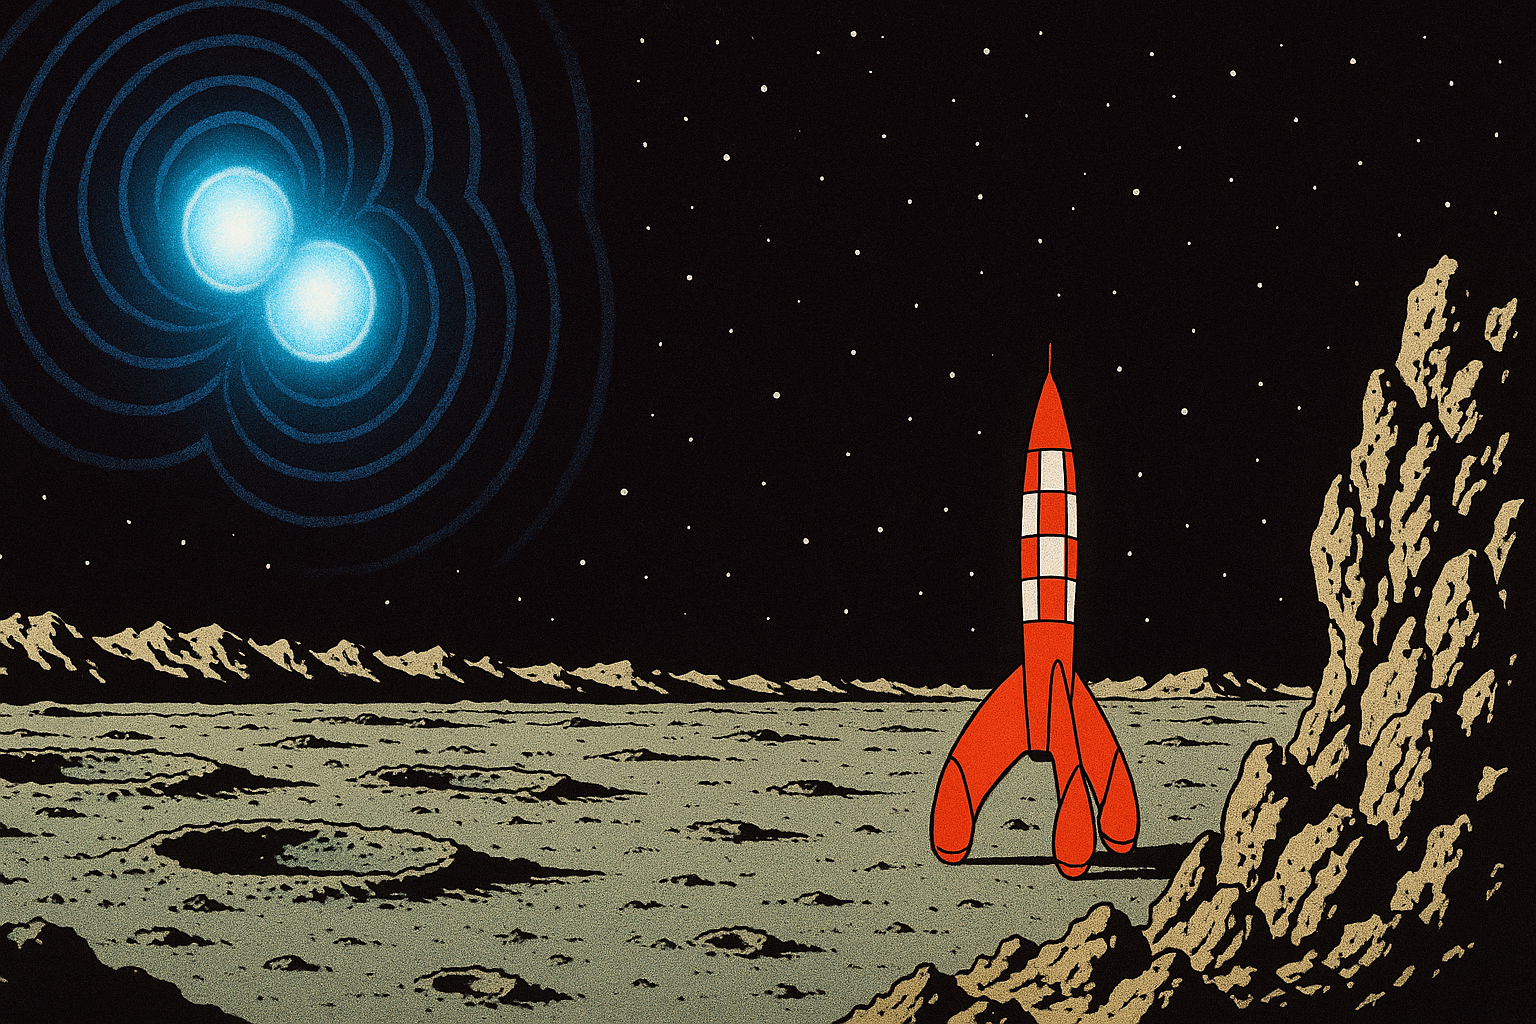
\includegraphics[width=\paperwidth,height=\paperheight]{tintin_BNS_2.png}}}

\begin{frame}[plain, noframenumbering]

  \begin{tikzpicture}[remember picture,overlay]
    \node[fill=customblue, fill opacity=0.75, text opacity=1, rounded corners=10pt, inner sep=15pt] at (current page.center) {
      \begin{minipage}{0.8\textwidth}
        \centering
        \textbf{GPU-accelerated multimessenger inference: applications and prospects}\\[1.5ex]
        \normalsize Thibeau Wouters, Peter T. H. Pang \\[0.5ex]
        \github \quad \linkedin \quad \myemail
      \end{minipage}
    };
  \end{tikzpicture}

  \vspace{7cm}

  \begin{columns}
  \column{0.35\textwidth}
  \begin{figure}
    \centering
    \vspace{1.5mm}
    
\includegraphics[width=0.75\linewidth]{utrecht-university.png}
  \end{figure}
  \column{0.35\textwidth}
  \begin{figure}
    \centering
    
\includegraphics[width=0.75\linewidth]{Nikhef_logo-transparent.png}
  \end{figure}
\end{columns}

\end{frame}
}

\begin{frame}
\frametitle{Table of Contents}
\tableofcontents[hideallsubsections]
\end{frame}

%---------------------------------------------------------
\section{Introduction}
%---------------------------------------------------------

\begin{frame}{Neutron stars}

  \def\x{3mm}

  \begin{itemize}
    \item Neutron stars: supernova remnants, densest matter in the universe

    \item $m \sim 1.2 - 2.3 M_\odot$, $R \sim 10-13$ km
  \end{itemize}

  \pause

  \centering
  \incfig[0.90\textwidth]{NS_above_Berlin}
\end{frame}


\begin{frame}{Equation of state}

  \def\x{3mm}

  Neutron stars probe the high-density part of the \blue{equation of state} (EOS) of dense nuclear matter~\smallcite{Koehn:2024set}

  \vspace{\x}

  \begin{figure}
    \centering
    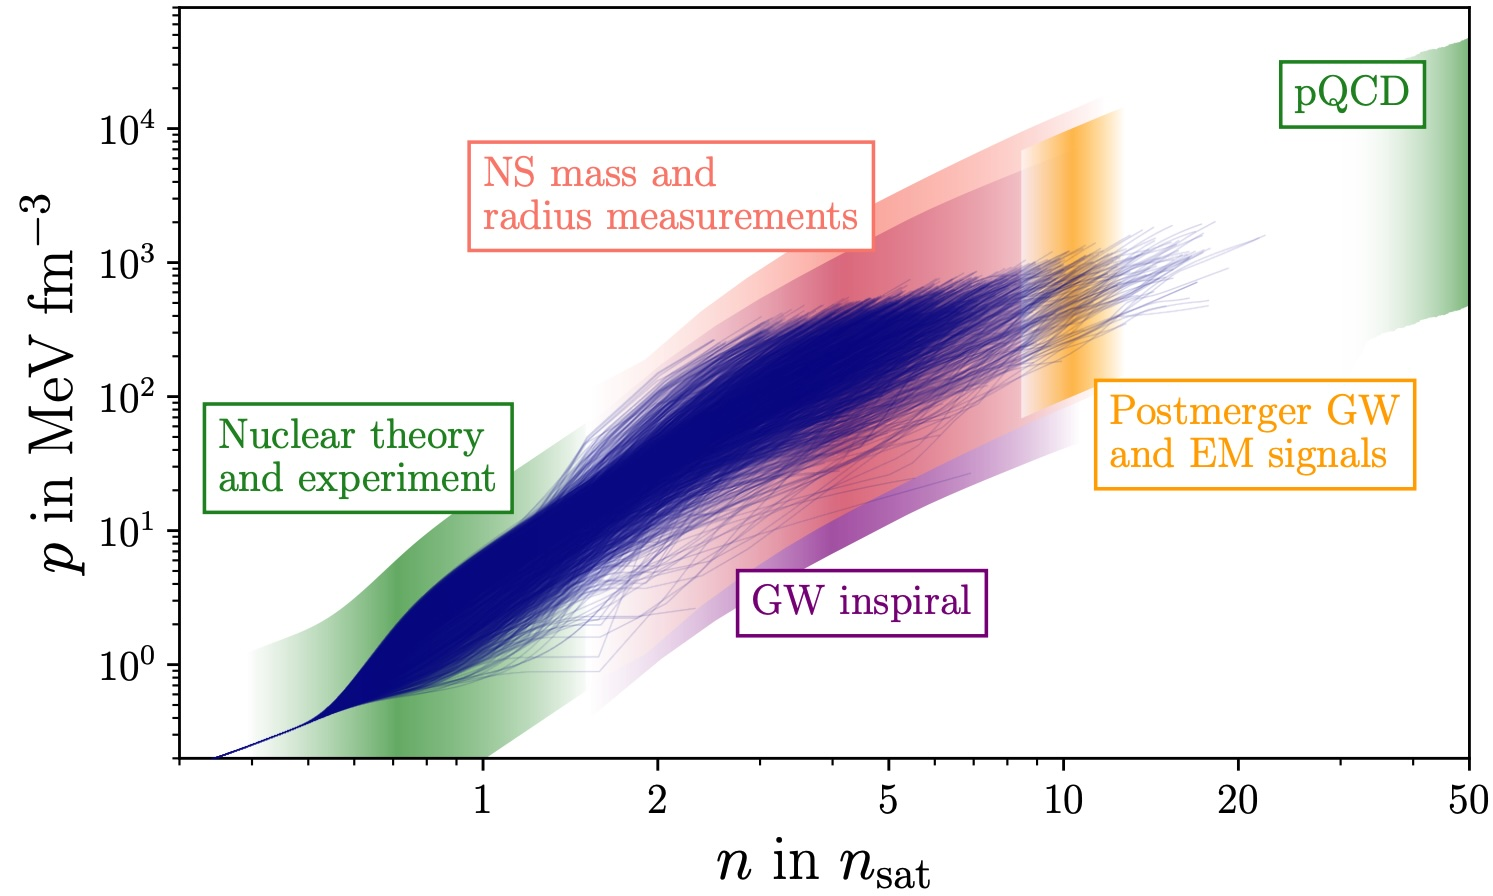
\includegraphics[width=0.85\linewidth]{Koehn_EOS.jpg}
  \end{figure}
\end{frame}


\begin{frame}{Multimessenger astrophysics: GW170817}

  \def\x{2mm}

  Neutron star mergers emit gravitational waves \emph{and} electromagnetic radiation: GW170817~\smallcite{LIGOScientific:2017vwq, LIGOScientific:2017zic}

  \only<1>{
    \begin{figure}
      \centering
      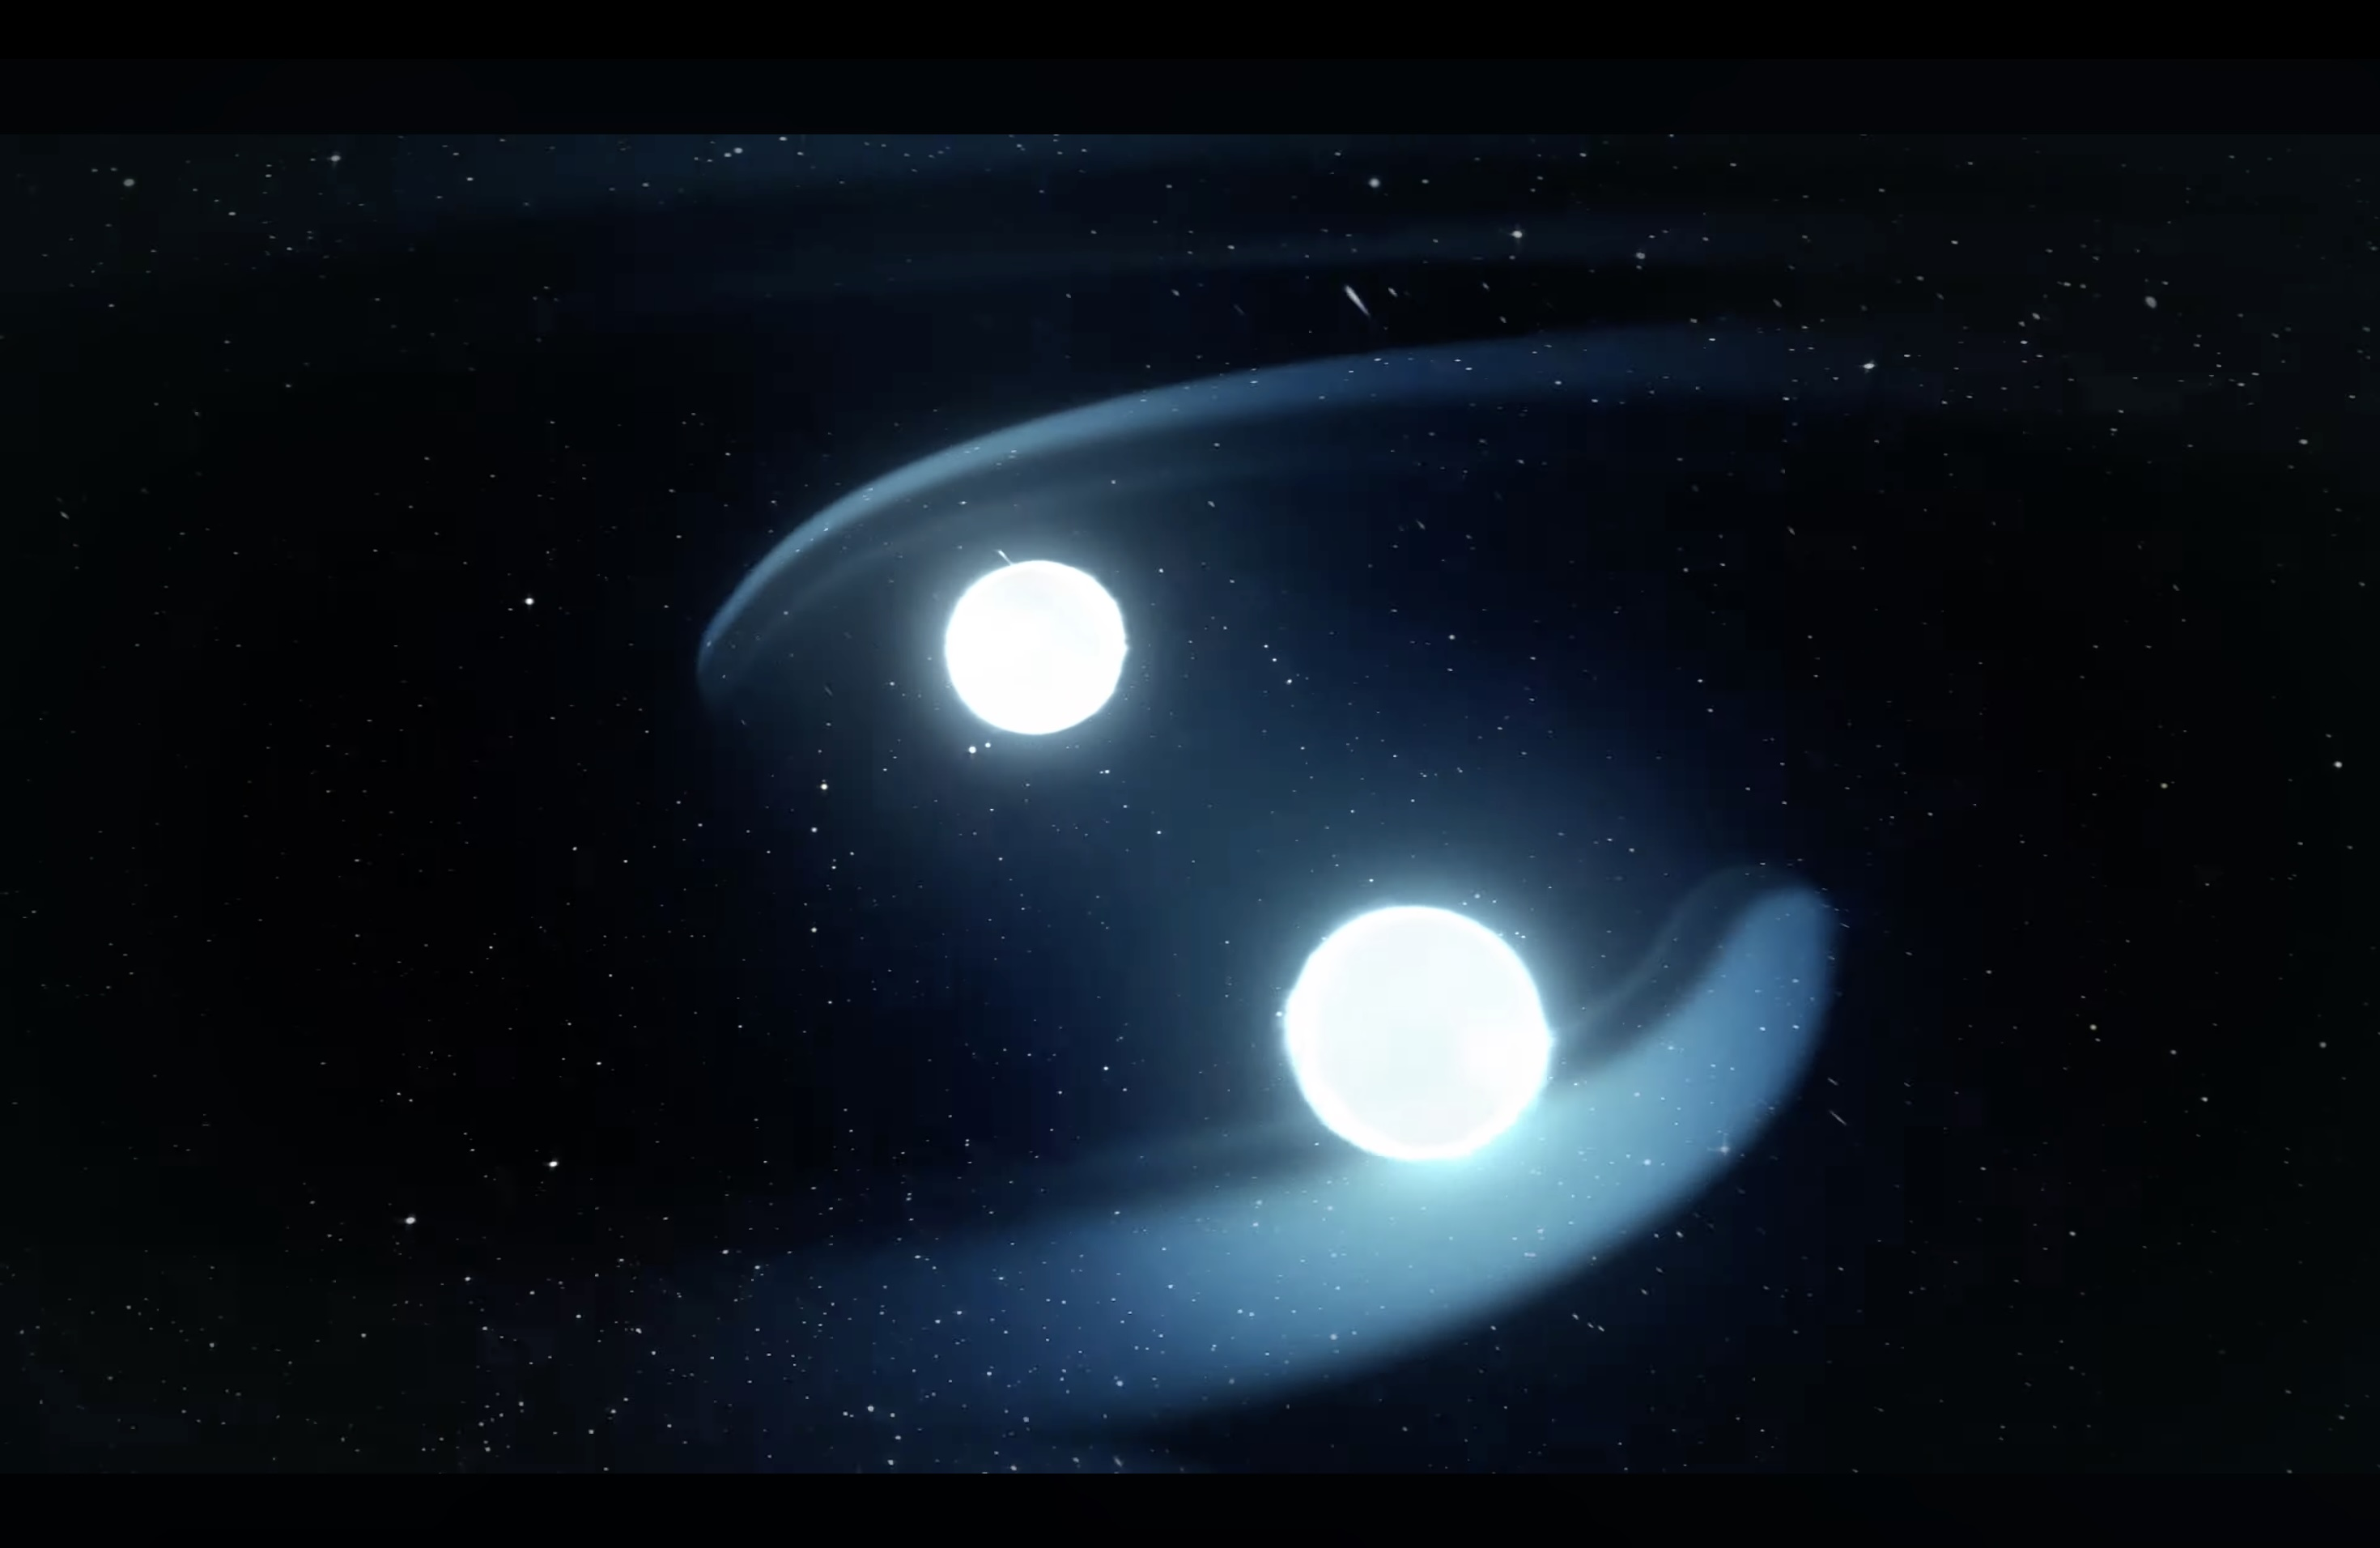
\includegraphics[width=0.95\linewidth]{GW170817_inspiral.jpg}
    \end{figure}
  }

  \only<2>{
    \begin{figure}
      \centering
      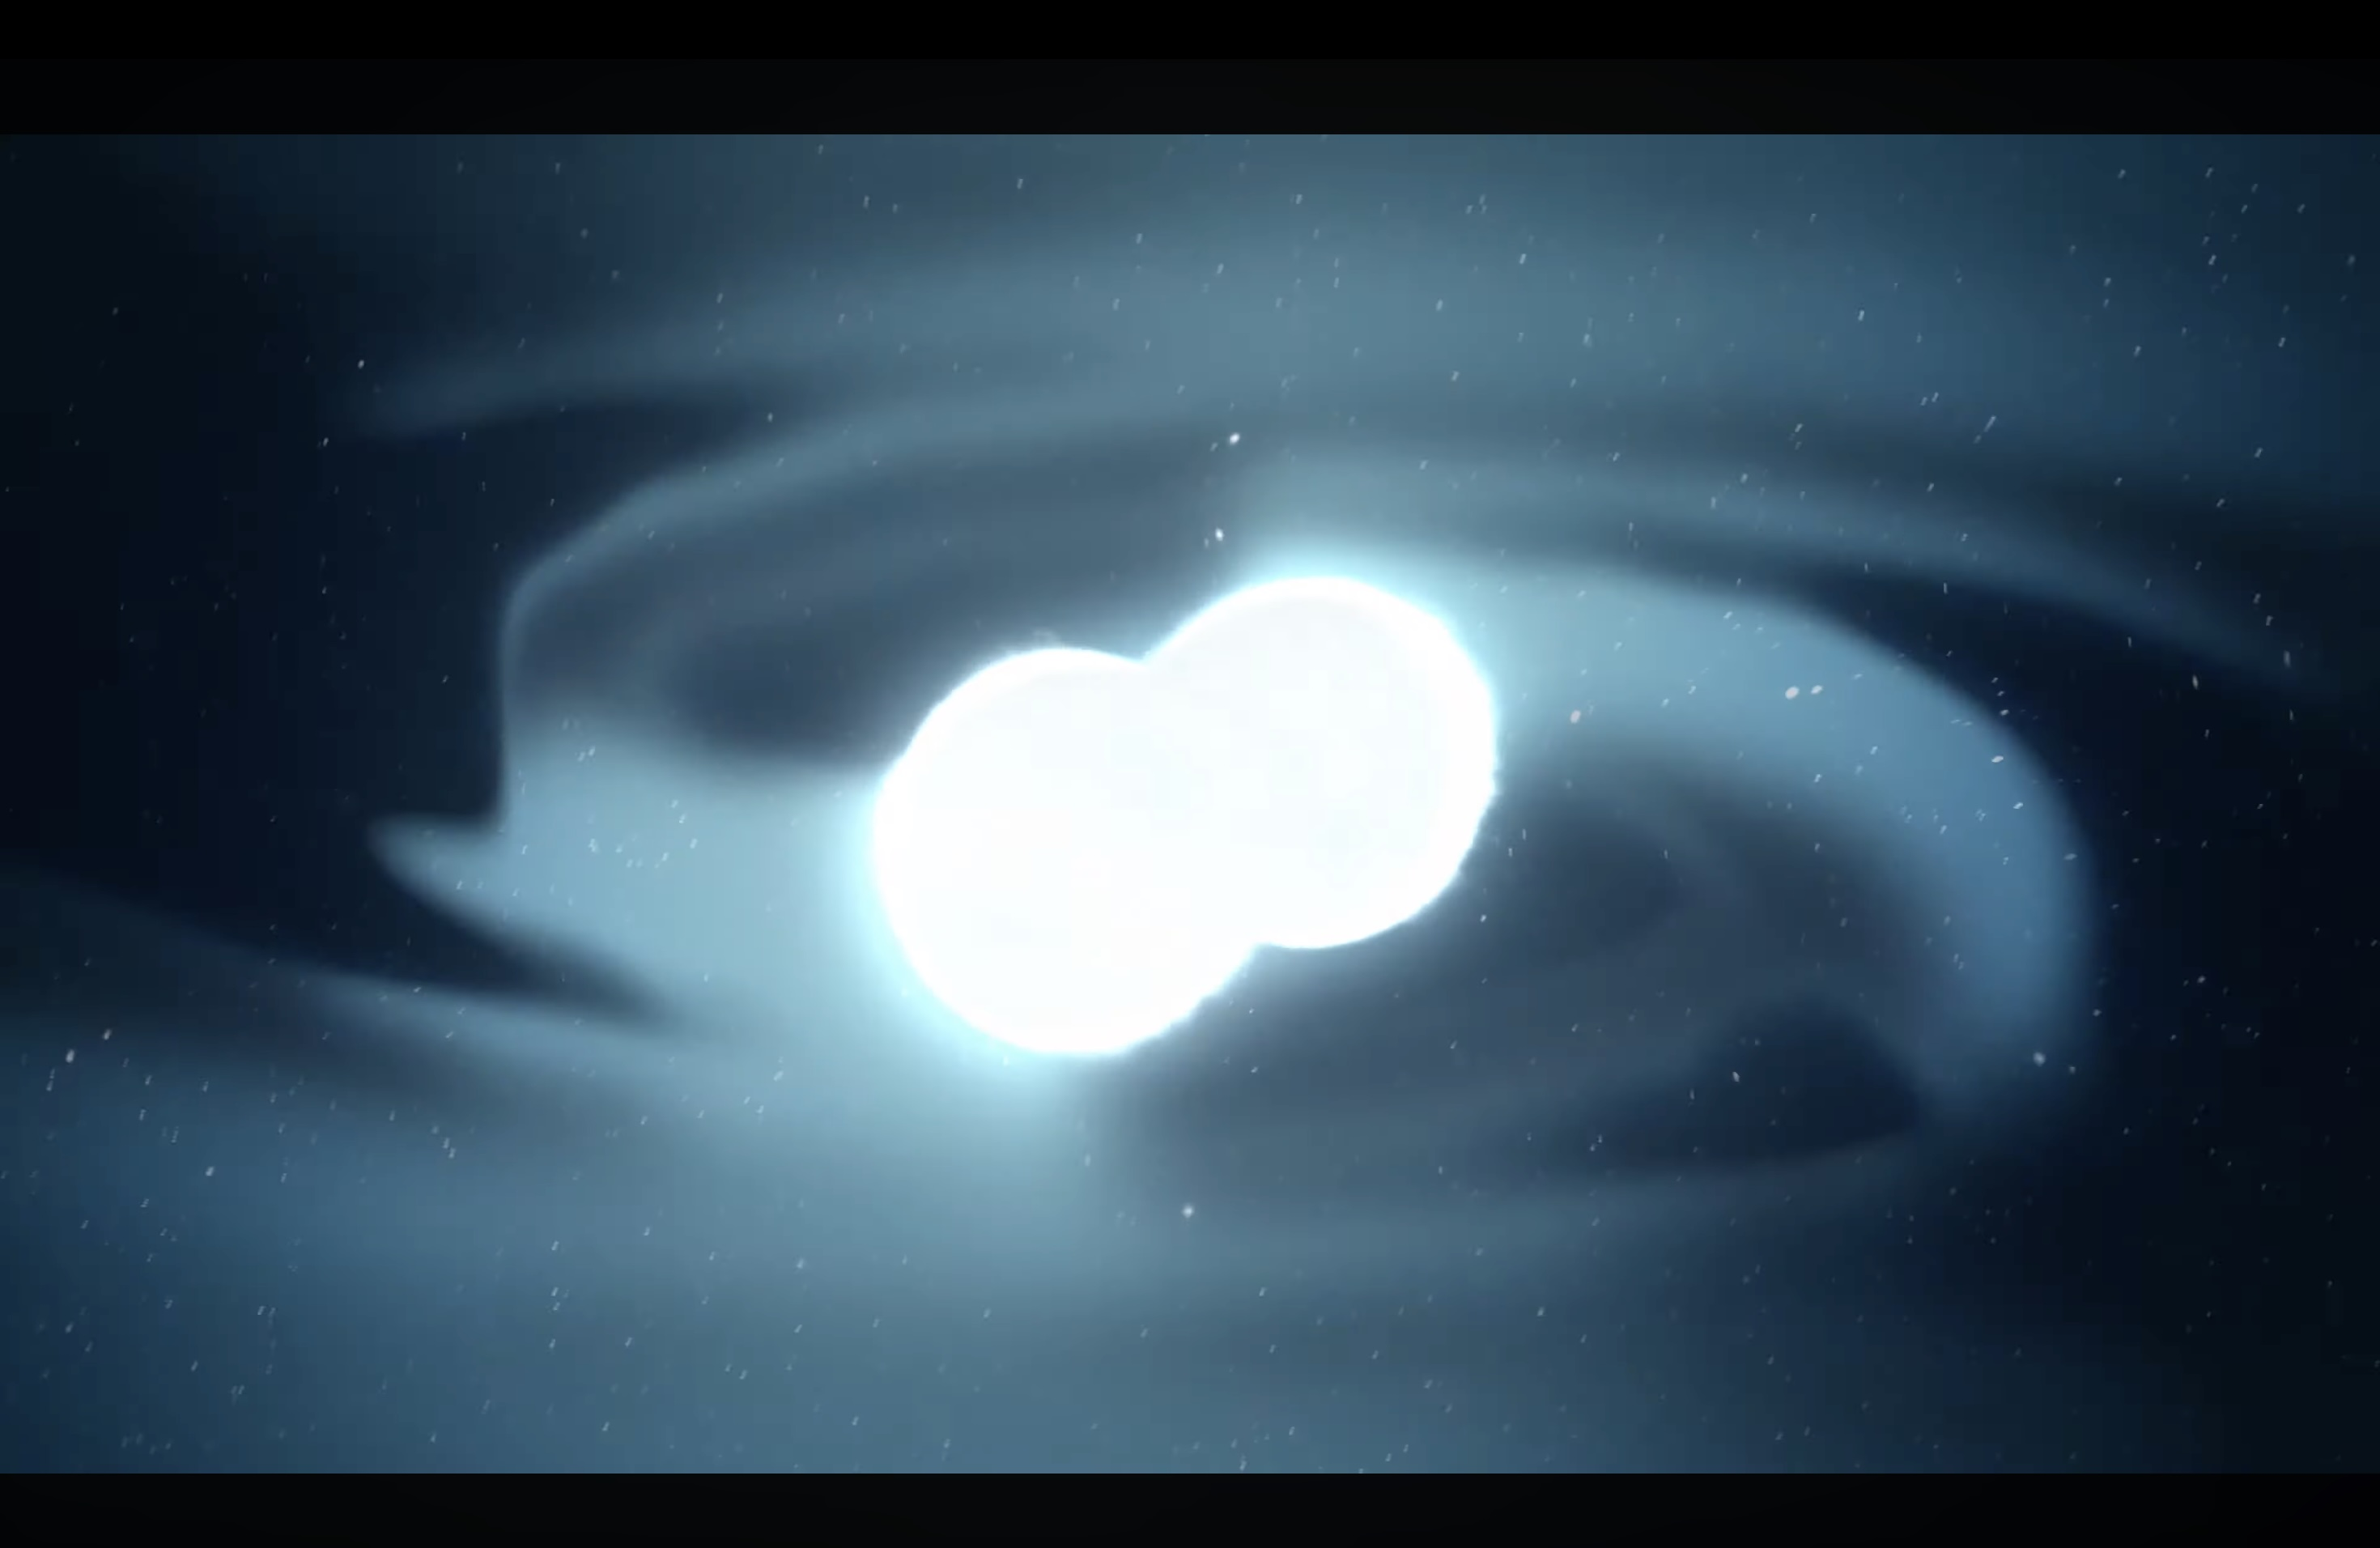
\includegraphics[width=0.95\linewidth]{GW170817_merger.jpg}
    \end{figure}
  }

  \only<3>{
    \begin{figure}
      \centering
      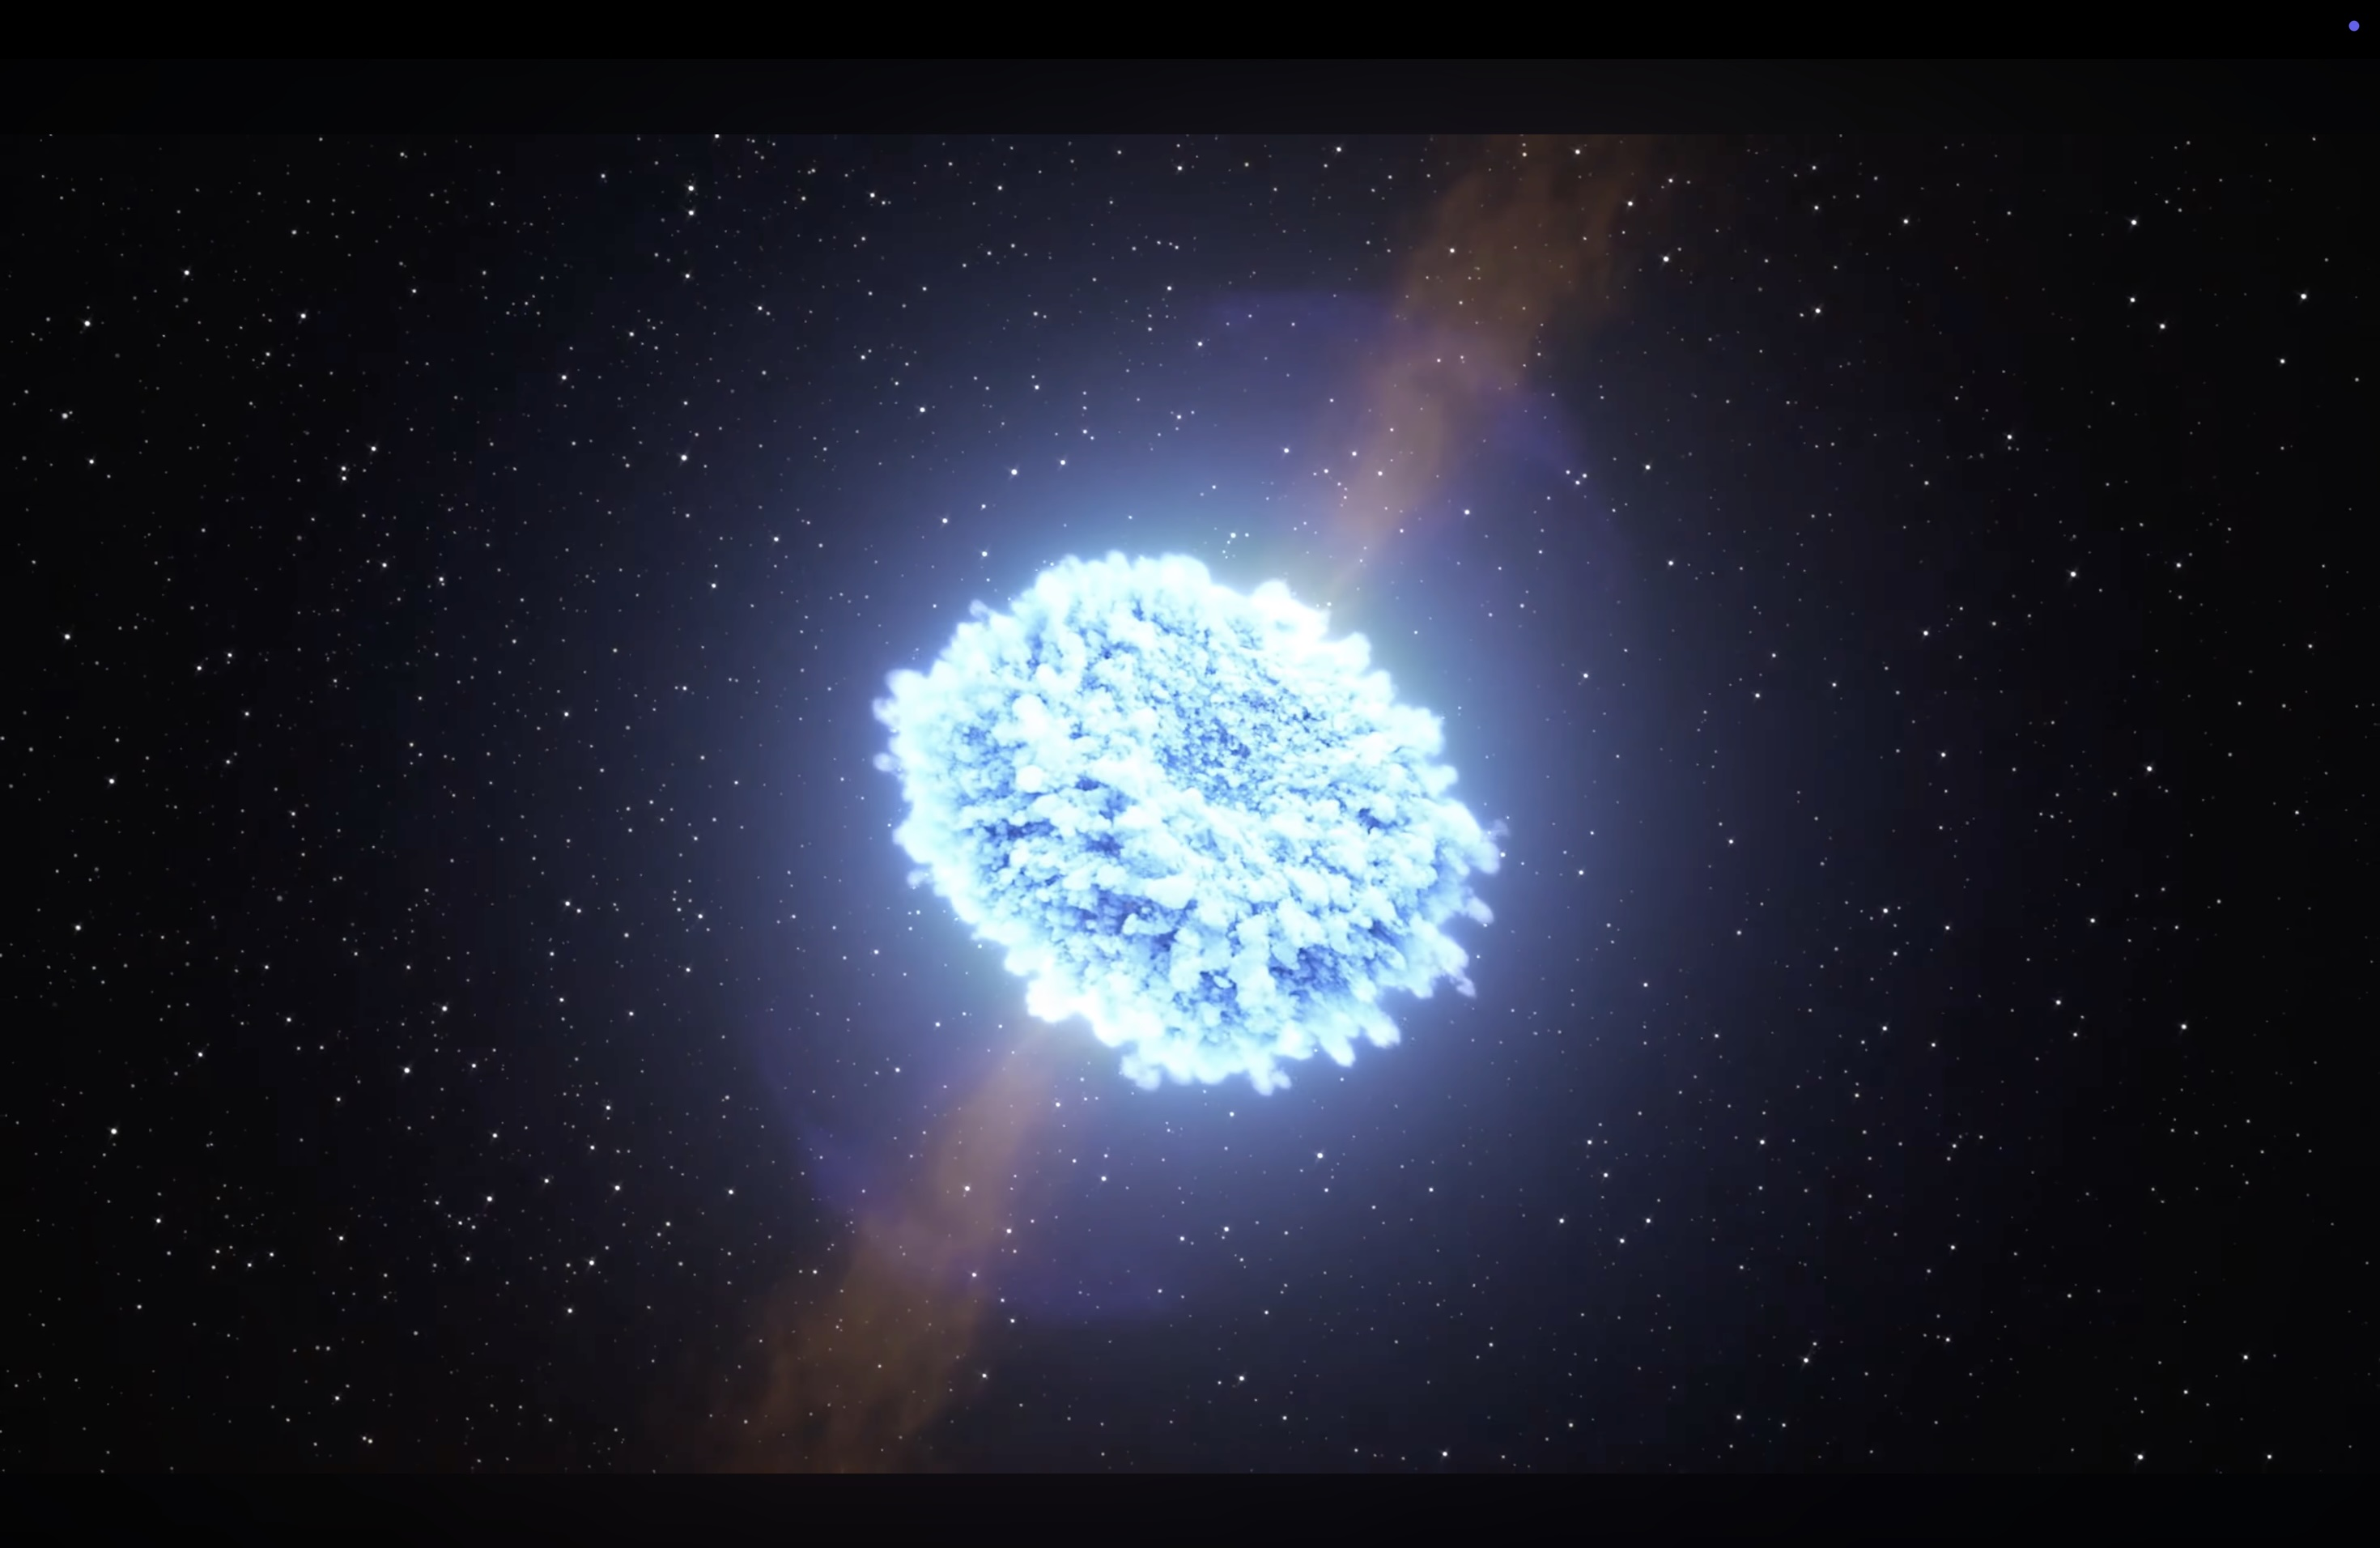
\includegraphics[width=0.95\linewidth]{GW170817_KN.jpg}
    \end{figure}
  }

\end{frame}


\begin{frame}{Tidal deformability}

  \def\x{4mm}

  \begin{itemize}
    \item Neutron stars are tidally deformed in a binary: quantified by $\Lambda$

    \vspace{\x}

    \item Affects phase of gravitational wave: $\Lambda = \Lambda(m, {\rm EOS})$

    \vspace{\x}

    \item Gravitational waves give $p(m_1, m_2, \Lambda_1, \Lambda_2 | d)$ for EOS inference
  \end{itemize}

  \vspace{\x}

  \centering
  \incfig[\textwidth]{tidal}
\end{frame}


\begin{frame}{Parameter estimation: Bayesian inference}

  \def\x{5mm}

  How do we ``measure'' source parameters $\theta$ from data $d$?

  \vspace{\x}
  \pause

  Bayesian inference:
  \begin{equation*}
    p(\theta|d) = \frac{p(d|\theta)\, p(\theta)}{p(d)} = \frac{\rm{likelihood} \times \rm{prior}}{\rm{evidence}}
  \end{equation*}

  \vspace{\x}
  \pause

  Ingredients:
  \begin{itemize}
    \item Posterior: intractable, needs stochastic samplers
    \begin{itemize}
      \item MCMC, nested sampling, sequential Monte Carlo
    \end{itemize}

    \item Prior: encode beliefs about parameters

    \item Likelihood: \red{computational bottleneck}

    \item Evidence: model selection
  \end{itemize}
\end{frame}


\begin{frame}{Connecting multimessenger data to the EOS}

  \def\x{2mm}
  \def\y{5mm}

  \begin{itemize}
    \item EOS determined with Bayesian inference:
    \begin{align*}
      p(\thetaeos | d ) &\propto \red{p(d | \thetaeos)} \, p(\thetaeos) \\
      \rm{posterior} &\propto \rm{\red{likelihood}} \times \rm{prior}
    \end{align*}

    \vspace{\x}

    \item Solve TOV equations to predict NS properties ($M$, $R$, $\Lambda$) from EOS
  \end{itemize}

  \vspace{\y}

  \centering
  \incfig[0.95\textwidth]{NS_likelihood}

\end{frame}


\begin{frame}{EOS parametrization}

  \def\x{2mm}
  \def\y{1mm}

  Flexible EOS models $\rightarrow$ \red{high-dimensional} parameter space

  \vspace{\y}
  \begin{itemize}
    \item $\tfrac12 n_{\rm{sat}} \leq n \leq n_{\rm{break}}$: Metamodel, nuclear physics inspired

    \vspace{\x}

    \item $n > n_{\rm{break}}$: agnostic speed-of-sound extension

    \vspace{\x}

    \item $>26$ parameters $\thetaeos$
  \end{itemize}

  \centering
  \incfig[0.825\textwidth]{EOS_parametrizion}
\end{frame}


\begin{frame}{Motivation: Why GPU-accelerated inference?}

  \def\x{4mm}
  \def\y{1mm}

  \begin{itemize}
    \item Studies bound by computational feasibility

    \vspace{\x}
    \pause
    
    \item Scientific progress is driven by algorithmic and software development
    
    \vspace{\x}
    \pause

    \item Scientific computing: traditionally \blue{CPU-based} Python
    \begin{itemize}
      \vspace{\y}
      \item \textsc{numpy}, \textsc{scipy}, \textsc{bilby}, ...
    \end{itemize}
    
    \pause
    \vspace{\x}
    
    \item AI boom: enabled by \red{GPU acceleration}
  \end{itemize}
  
  \pause
  \vspace{\x}

  \begin{tcolorbox}[colback=red!10!white, colframe=red!80!black, coltext=black]
  \textbf{Question:} Can we leverage GPU acceleration for multimessenger data analysis without compromising accuracy?
  \end{tcolorbox}
\end{frame}

% \begin{frame}{Why scalable inference?}

%   \def\x{4mm}
%   \def\y{1mm}

%   \vspace{-3mm}

%   \begin{tcolorbox}[colback=jaxbluedarkcolor!15!white, colframe=jaxbluedarkcolor!80!black, coltext=black]
%   \textbf{Why?} Make multimessenger inference tractable 
%   \begin{itemize}
%     \vspace{\y}
%     \item Prepare for future detectors (Einstein Telescope)
%     \vspace{\y}
%     \item Understand systematics through simulated data
%     \vspace{\y}
%     \item Probe novel effects (complex models)
%   \end{itemize}
%   \end{tcolorbox}

%   \pause
%   \vspace{\y}

%   \begin{tcolorbox}[colback=jaxgreendarkcolor!15!white, colframe=jaxgreendarkcolor!80!black, coltext=black]
%   \textbf{How?} Without compromises to accuracy
%   \begin{itemize}
%     \vspace{\y}
%     \item GPU hardware + differentiable programming (\textsc{jax})
%   \end{itemize}
%   \end{tcolorbox}

%   \pause
%   \vspace{\y}

%   \begin{tcolorbox}[colback=jaxthreecolor!15!white, colframe=jaxthreecolor!80!black, coltext=black]
%   \textbf{What?} GPU-accelerated Bayesian inference of BNS mergers and the EOS
%   \end{tcolorbox}

% \end{frame}


%---------------------------------------------------------
\section{Methods}
%---------------------------------------------------------

\begin{frame}{\textsc{jax}}

  \def\x{5mm}
  \def\y{1mm}

  \begin{columns}
    \begin{column}[t]{0.88\linewidth}
      \textsc{jax}~\ghlink{jax-ml/jax}~\smallcite{jax2018github}: \red{High-performance} numerical computing in Python
    \end{column}
    \begin{column}[t]{0.10\linewidth}
      \vspace{0pt}
      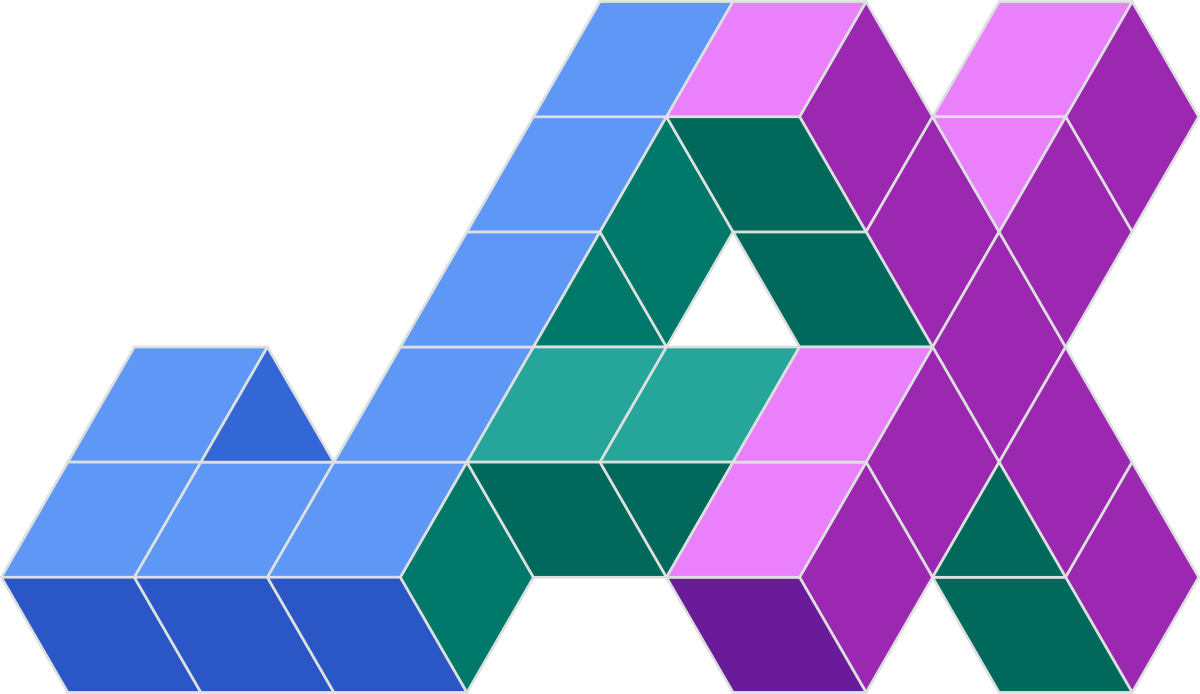
\includegraphics[width=0.85\linewidth]{jax.png}
    \end{column}
  \end{columns}

  \vspace{\x}
  \pause

  Gamechangers:
  \begin{itemize}
    \vspace{\y}
    \item GPU accelerators: run Python on hardware accelerators

    \vspace{\y}

    \item Composable function transformations:
    \begin{itemize}
      \item \jaxjit: just-in-time compilation
      \item \jaxgrad: automatic differentiation (exact, fast)
      \item \jaxvmap: vectorization / batch processing
    \end{itemize}
  \end{itemize}

  \pause
  \vspace{3mm}

  Example gradient descent on \textit{any} loss function:
  \begin{equation*}
    \boldtheta \leftarrow \boldtheta + \alpha\, \jaxvmap\!\left(\jaxjit(\jaxgrad(\mathcal{L}(\boldtheta)))\right)
  \end{equation*}

\end{frame}

\begin{frame}{Sequential Monte Carlo (SMC)}

  \def\x{4mm}
  \def\y{2mm}

  \begin{itemize}
    \item Compute posterior and Bayesian evidence
    
    \vspace{\y}

    \item Evolve swarm of particles through distributions~\smallcite{Williams:2025szm}:
    \begin{equation*}
      p_t(\theta | d) \propto p(d | \theta)^{\beta_t} p(\theta) \, , \quad \beta_t \in [0, 1] \, .
    \end{equation*}

    \vspace{\y}

    \item Parallelizable: efficient on GPU
  \end{itemize}

  \begin{figure}
    \centering
    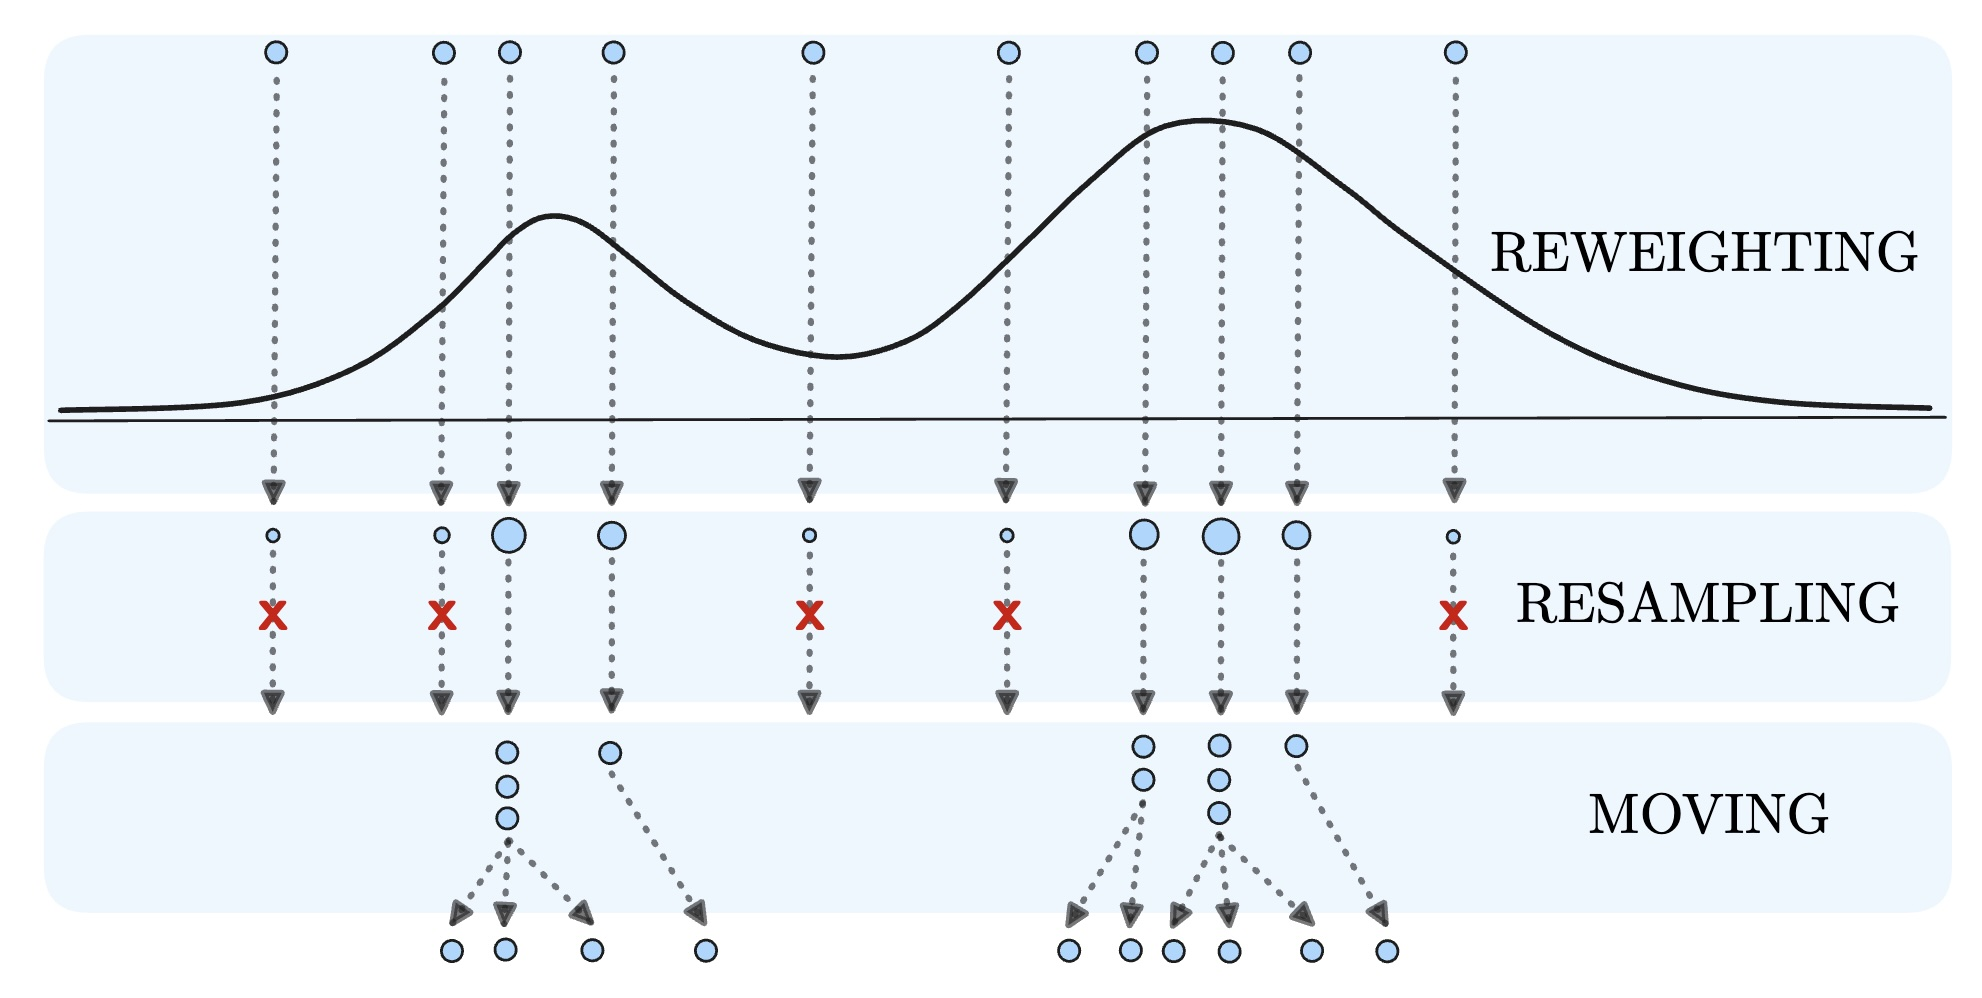
\includegraphics[width=0.75\textwidth]{SMC_diagram.jpg}
  \end{figure}
\end{frame}

\begin{frame}{\textsc{Jim}: GPU-accelerated GW parameter estimation}

  \def\x{3mm}
  \def\z{3mm}

  \textsc{Jim}~(\ghlink{GW-JAX-Team/jim}~\texttt{GW-JAX-Team/jim}): gravitational wave parameter estimation

  \only<2>{
    \vspace{2mm}
    \begin{columns}
      \column{0.50\textwidth}
    
      \begin{itemize}
        \item Re-analyze GWTC-3 and GWTC-4 events
        
        \vspace{\z}
        
        \item Support different samplers
        
        \vspace{\z}

        \item Matches \textsc{bilby}
        
        \vspace{\z}
        
        \item All $\sim2\times$ -- $10\times$ faster than \textsc{bilby} on GPU
      \end{itemize}

      \column{0.50\textwidth}
      
      \centering
      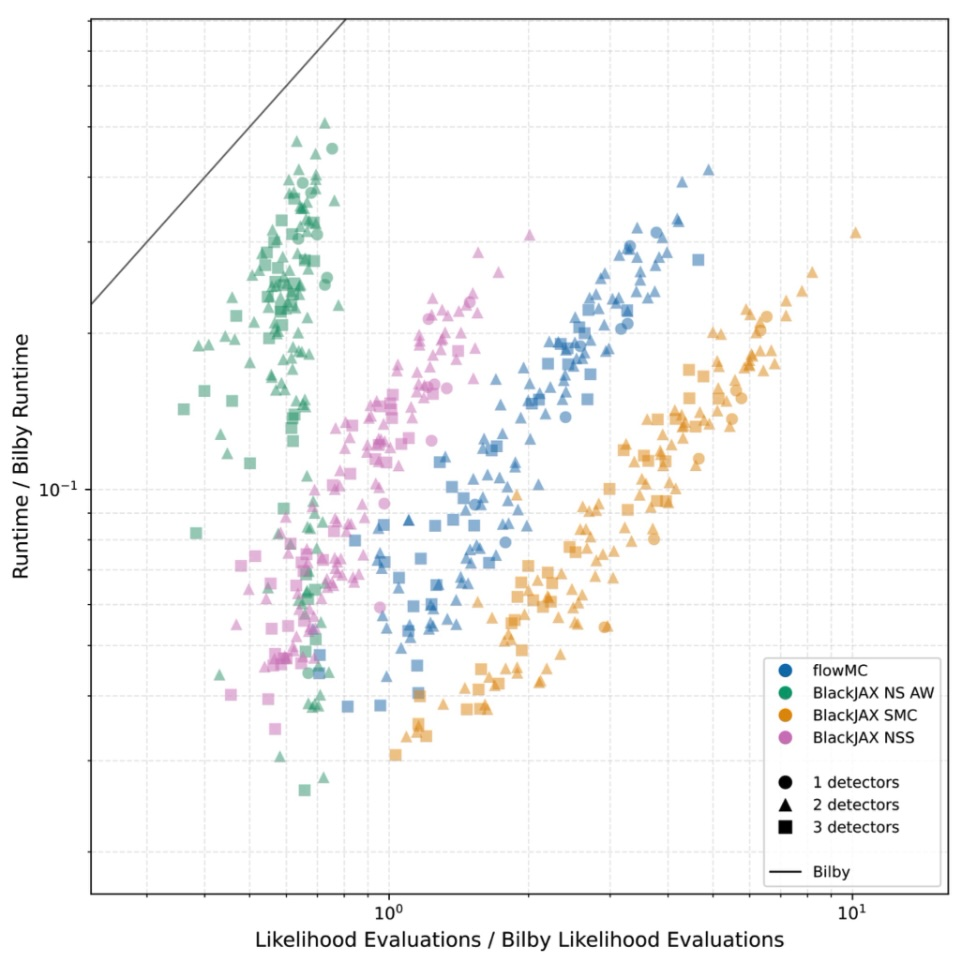
\includegraphics[width=\linewidth]{jim_performance_now.jpg}
      \tiny Credits: Thomas C. K. Ng \normalsize
    \end{columns}
  }

\end{frame}

%---------------------------------------------------------
\section{\textsc{jester}: EOS Inference}
%---------------------------------------------------------

\begin{frame}{\textsc{jester}: JAX-accelerated EOS inference}

  \def\x{5mm}
  \def\y{1mm}

  \vspace{-4mm}

  \begin{columns}[t]
    \column{0.80\textwidth}
    \begin{itemize}
      \item Hierarchical EOS inference in JAX~\smallcite{Wouters:2025zju}
      \item GPU-accelerated TOV solvers and samplers
      \item \ghlink{nuclear-multimessenger-astronomy/jester}~\texttt{nuclear-multimessenger-astronomy/jester}
    \end{itemize}

    \column{0.20\textwidth}
    \begin{figure}
      \centering
      
\includegraphics[scale=0.05]{JESTER_logo.png}
    \end{figure}
  \end{columns}

  \vspace{\x}
  \pause

  Currently available:
  \begin{itemize}
    \vspace{\y}

    \item EOS models:
    \begin{itemize}
      \item Fixed crust + Metamodel + speed-of-sound (MM+CSE)
      \item Fixed crust + spectral expansion
    \end{itemize}

    \vspace{\y}

    \item Samplers:
    \begin{itemize}
      \item Nested sampling (NS)
      \item Sequential Monte Carlo (SMC)
    \end{itemize}

    \vspace{\y}

    \item Likelihoods: nuclear physics \& multimessenger data
  \end{itemize}
\end{frame}


%---------------------------------------------------------
\section{Results}
%---------------------------------------------------------

\subsection{Einstein Telescope projections}

\begin{frame}{Einstein Telescope}

  \def\x{4mm}
  \def\y{2mm}

  Simulated study for Einstein Telescope~\smallcite{ET:2019dnz}:
  \begin{itemize}
    \vspace{\y}
    \item 100 loudest binary neutron star mergers from 1 year~\cite{Branchesi:2023mws}
  \end{itemize}

  \pause
  % \vspace{\x}

  \begin{figure}
    \centering
    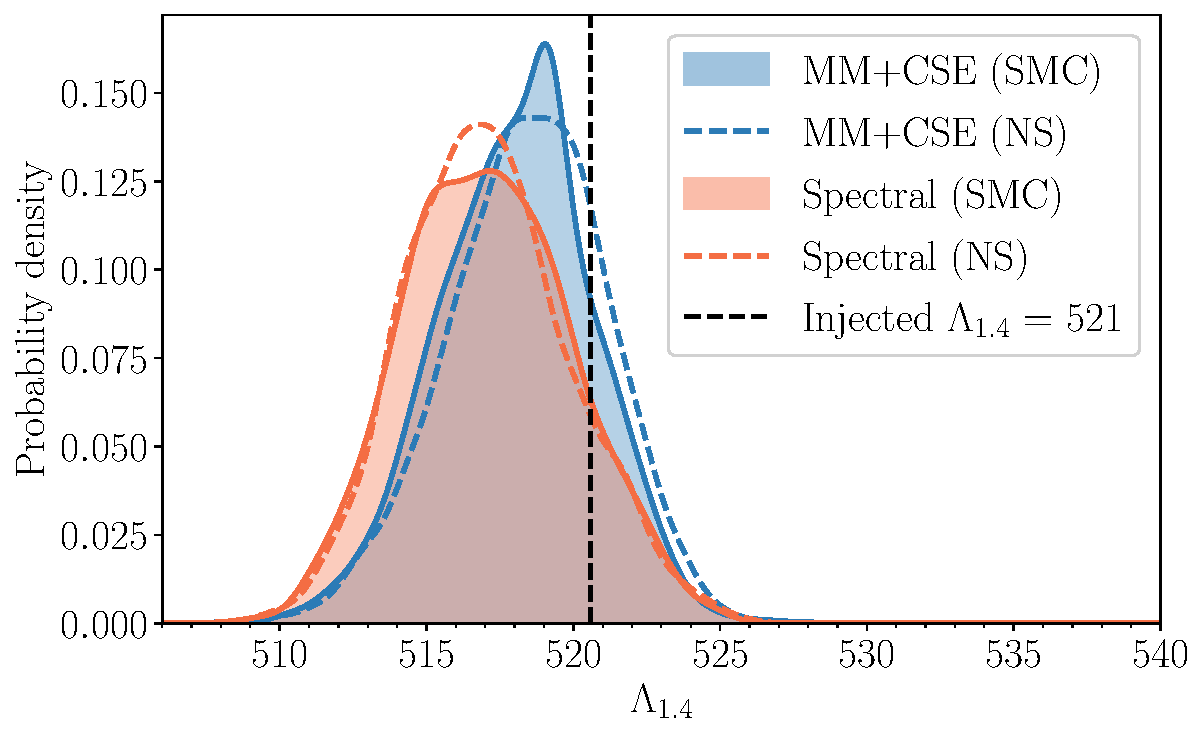
\includegraphics[width=0.88\textwidth]{ET_ET_lambda14_comparison.pdf}
  \end{figure}

\end{frame}


\begin{frame}{Einstein Telescope}

  \begin{figure}
    \centering
    
\includegraphics[width=0.88\textwidth]{ET_ET_r14_comparison.pdf}
  \end{figure}

  \begin{itemize}
    \item Different EOS parametrizations: different uncertainties on $R_{1.4}$
    \item Samplers consistent
  \end{itemize}

\end{frame}


\begin{frame}{Einstein Telescope: runtimes}

  Scalable inference with many high-SNR sources: \red{enable projection studies}

  \vspace{4mm}

  \begin{table}[h]
    \centering
    \renewcommand{\arraystretch}{1.4}
\begin{tabular}{p{4.5cm}cc}
    \hline
    EOS model & Sequential Monte Carlo & Nested Sampling \\
    \hline
    Metamodel\newline + speed-of-sound & 1h 24m & 13h 07m \\
    Spectral decomposition & 20m 10s & 1h 11m \\
    \hline
\end{tabular}

    \caption{Sampling time on 1 NVIDIA H100 GPU.}
  \end{table}

\end{frame}


\subsection{Pressure anisotropy}

\begin{frame}{Pressure anisotropy in neutron stars}

  \def\x{3mm}
  \def\y{1mm}

  \vspace{-3mm}

  \begin{columns}
    \begin{column}{0.55\textwidth}
      \begin{itemize}
        \item Standard TOV: assumes \blue{isotropic pressure} ($p_r = p_t$)

        \vspace{\x}

        \item Physical mechanisms can violate this (pion/kaon condensation, magnetic fields, superfluidity)

        \vspace{\x}

        \item Anisotropy parameter $\sigma \equiv p_r - p_t$; model:
        \begin{equation*}
          \sigma = \red{\gamma} \,\frac{2m p_r}{r}
        \end{equation*}
      \end{itemize}
    \end{column}
    \begin{column}{0.44\textwidth}
      \begin{figure}
        \centering
        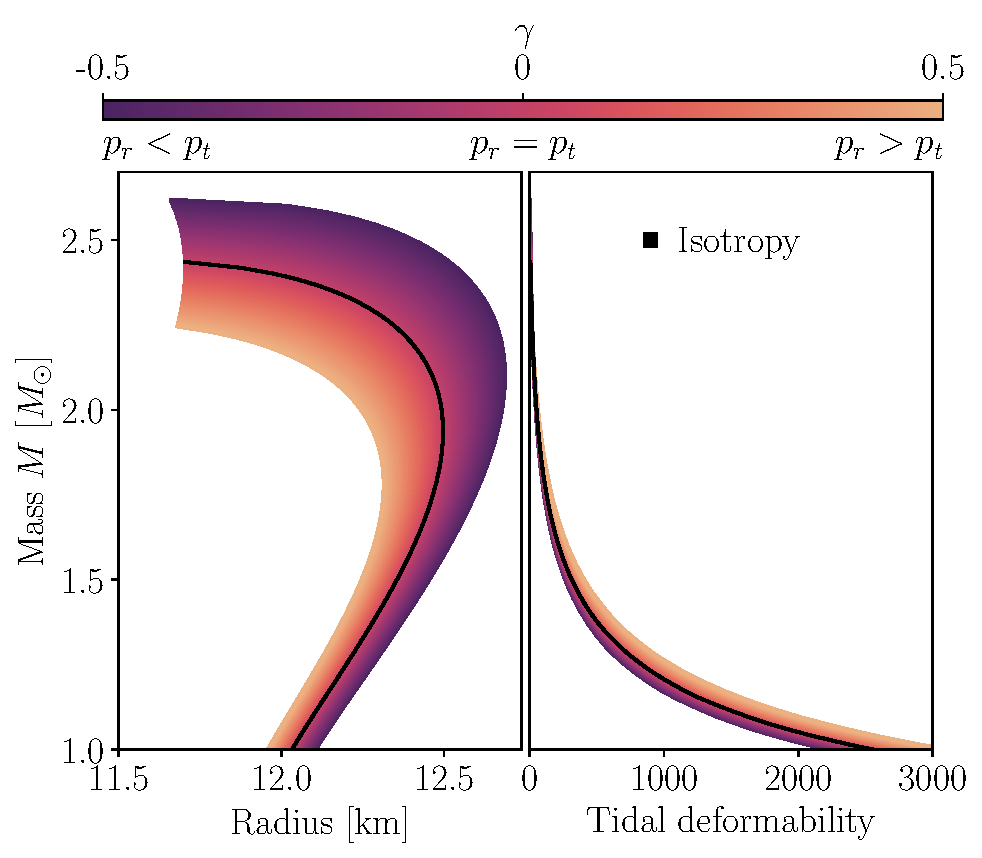
\includegraphics[width=0.99\linewidth]{pressure_anistropy_demo_art.pdf}
      \end{figure}
    \end{column}
  \end{columns}

  \vspace{\x}

  \begin{tcolorbox}[colback=blue!5!white, colframe=blue!75!black]
    Key question: can we ``measure'' anisotropy ($\gamma \neq 0$) with current data?
  \end{tcolorbox}

\end{frame}


\begin{frame}{Measuring anisotropy with \textsc{jester}}

  \def\x{3mm}
  \def\y{1mm}

  Modified TOV equations with anisotropic pressure~\smallcite{Pang:2025fes}:
  \begin{itemize}
    \vspace{\y}
    \item $\gamma$ enters the structure equations and tidal deformability
    \vspace{\y}
    \item Implemented as additional free parameter in \textsc{jester}
  \end{itemize}

  \pause
  \vspace{\x}

  Hierarchical Bayesian inference across multiple neutron stars:
  \begin{itemize}
    \vspace{\y}
    \item Multimessenger data: GW + NICER + nuclear theory
    \vspace{\y}
    \item $\gamma$ allowed to vary \emph{per star} (breaks EOS degeneracy)
    \vspace{\y}
    \item Model selection: anisotropic vs isotropic hypothesis
  \end{itemize}

\end{frame}


\begin{frame}{Anisotropy results~\smallcite{Pang:2025fes}}

  \def\x{3.5mm}

  \begin{columns}
    \begin{column}{0.58\textwidth}
      \begin{figure}
        \centering
        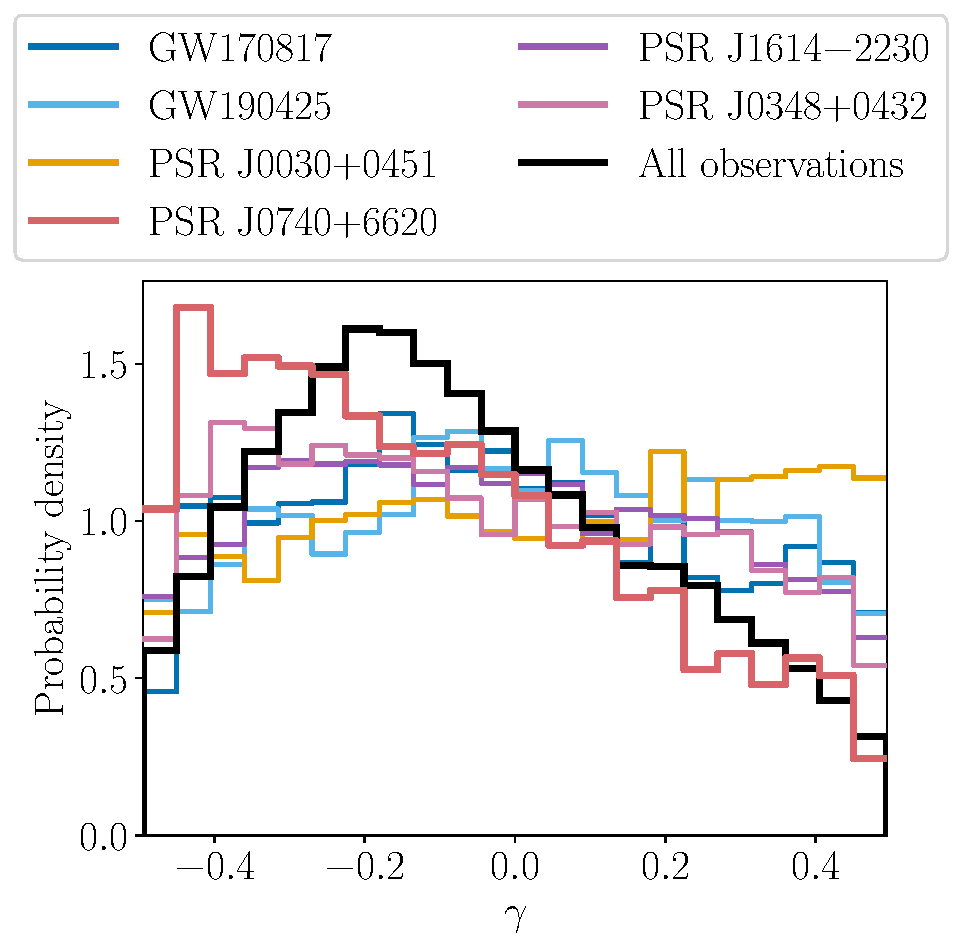
\includegraphics[width=0.99\linewidth]{individual_gamma_hist_noGaussian.pdf}
      \end{figure}
    \end{column}

    \begin{column}{0.41\textwidth}
      \begin{itemize}
        \item Preference for \red{negative} anisotropy

        \vspace{\x}

        \item Driven by \red{PSR J0740+6620} (NICER)

        \vspace{\x}

        \item Bayes factor $\gtrsim 3:1$ for anisotropy vs isotropy

        \vspace{\x}

        \item Evidence inconclusive, but anisotropy remains a useful probe
      \end{itemize}
    \end{column}
  \end{columns}

\end{frame}


%---------------------------------------------------------
\section{Conclusion}
%---------------------------------------------------------

\begin{frame}{Conclusion}

  \def\x{5mm}

  \begin{itemize}
    \item \textsc{jax}: GPU-accelerated Python

    \vspace{\x}

    \item \textsc{Jim}: GW parameter estimation in minutes

    \vspace{\x}

    \item \textsc{jester}: hierarchical EOS inference on GPU
    \begin{itemize}
      \item Multiple samplers (nested sampling, sequential Monte Carlo)
      \item Nuclear physics and multimessenger likelihoods
    \end{itemize}

    \vspace{\x}
    
    \item Applications:
    \begin{itemize}
      \item Projections for Einstein Telescope: scalable inference
      \item Anisotropy: probe structure of individual neutron stars
    \end{itemize}
  \end{itemize}

\end{frame}

{
\usebackgroundtemplate{\transparent{0.5}{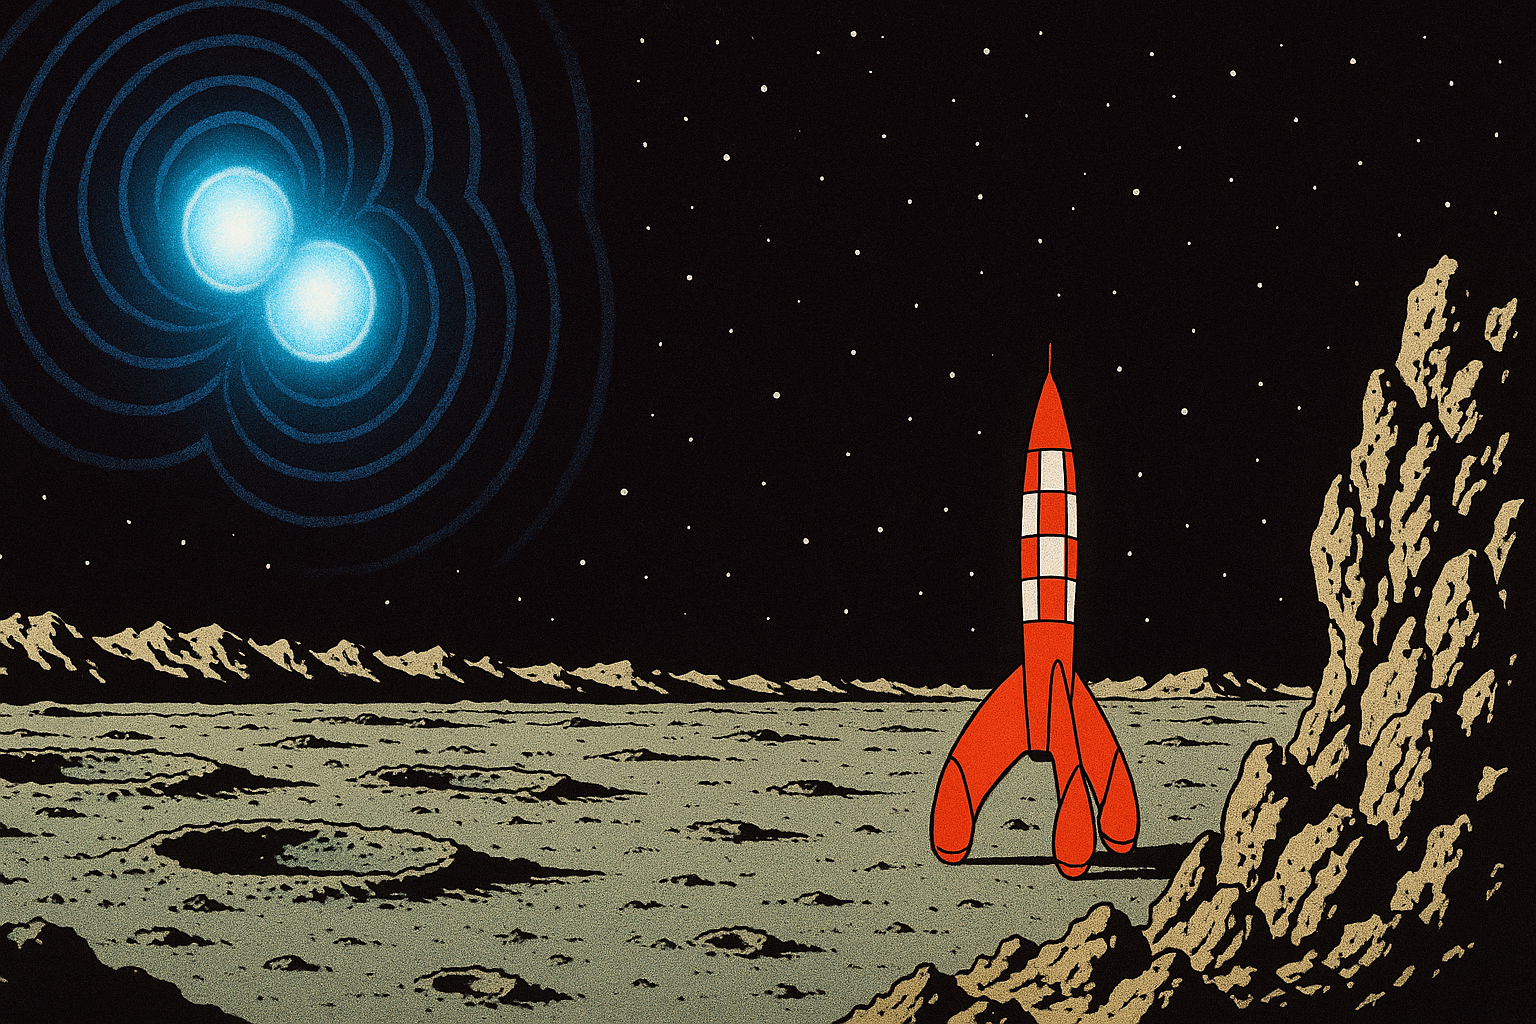
\includegraphics[width=\paperwidth,height=\paperheight]{tintin_BNS_2.png}}}

\begin{frame}[plain, noframenumbering]

  \begin{tikzpicture}[remember picture,overlay]
    \node[fill=customblue, fill opacity=0.75, text opacity=1, rounded corners=10pt, inner sep=15pt] at ([yshift=2cm]current page.center) {
      \begin{minipage}{0.8\textwidth}
        \centering
        \textbf{Thanks for listening!}\\[1ex]
        \normalsize Questions?
      \end{minipage}
    };
  \end{tikzpicture}

\end{frame}
}

\begin{frame}[allowframebreaks]{References}
  \printbibliography
\end{frame}

\end{document}
